\documentclass[a4paper,english,12pt]{article}
\usepackage{%
	amsfonts,%
	amsmath,%	
	etex,%
	amssymb,%
	amsthm,%
	babel,%
	bbm,%
	%biblatex,%
	caption,%
	centernot,%
	color,%
	enumerate,%
	epsfig,%
	epstopdf,%
	geometry,%
	graphicx,%
	hyperref,%
	latexsym,%
	mathtools,%
	multicol,%
	pgf,%
	pgfplots,%
	pgfplotstable,%
	pgfpages,%
	proof,%
	psfrag,%
	subfigure,%	
	tikz,%
	ulem,%
	url%
}	

\usepackage[mathscr]{eucal}
\usepgflibrary{shapes}
\usetikzlibrary{%
  arrows,%
	backgrounds,%
	chains,%
	decorations.pathmorphing,% /pgf/decoration/random steps | erste Graphik
	decorations.text,%
	matrix,%
  	positioning,% wg. " of "
  	fit,%
	patterns,%
  	petri,%
	plotmarks,%
  	scopes,%
	shadows,%
  	shapes.misc,% wg. rounded rectangle
  	shapes.arrows,%
	shapes.callouts,%
  	shapes%
}

\theoremstyle{plain}
\newtheorem{thm}{Theorem}[section]
\newtheorem{lem}[thm]{Lemma}
\newtheorem{prop}[thm]{Proposition}
\newtheorem{cor}[thm]{Corollary}

\theoremstyle{definition}
\newtheorem{defn}[thm]{Definition}
\newtheorem{conj}[thm]{Conjecture}
\newtheorem{exmp}[thm]{Example}
\newtheorem{assum}[thm]{Assumptions}
\newtheorem{axiom}[thm]{Axiom}

\theoremstyle{remark}
\newtheorem{rem}{Remark}
\newtheorem{note}{Note}

\newcommand{\norm}[1]{\left\lVert#1\right\rVert}
\newcommand{\indep}{\!\perp\!\!\!\perp}
\DeclarePairedDelimiter\abs{\lvert}{\rvert}%
%\DeclarePairedDelimiter\norm{\lVert}{\rVert}%
\newcommand{\tr}{\operatorname{tr}}
\newcommand{\R}{\mathbb{R}}
\newcommand{\Q}{\mathbb{Q}}
\newcommand{\N}{\mathbb{N}}
\newcommand{\E}{\mathbb{E}}
\newcommand{\Z}{\mathbb{Z}}
\newcommand{\B}{\mathscr{B}}
\newcommand{\C}{\mathcal{C}}
\newcommand{\T}{\mathscr{T}}
\newcommand{\F}{\mathcal{F}}
\newcommand{\G}{\mathcal{G}}
%\newcommand{\ba}{\begin{align*}}
%\newcommand{\ea}{\end{align*}}

\makeatletter
\def\th@plain{%
  \thm@notefont{}% same as heading font
  \itshape % body font
}
\def\th@definition{%
  \thm@notefont{}% same as heading font
  \normalfont % body font
}
\makeatother
\date{}

%opening
\title{Lecture-4: Queues and Compound Poisson Processes}
\author{Instructor-Parimal Parag \\
		Scribe- Vinay Kumar B R}
\date{January 21, 2016}
\begin{document}
\maketitle
\tableofcontents
\section{Queueing Theory}
\subsection{A preliminary example}
\par Consider the scenario of a bus stop or a movie ticket counter. Each person arrives to the queue at a random time and has to wait another random amount of time before he is serviced. A natural que(ue)stion to ask is regarding the expected total waiting time of all the people in the queue. To answer this question, we first formalize the idea of a queue.\\
\par Consider a queue where the customers are arriving according to a Poisson process of rate $\lambda$. Let $N(t)$ be the random variable for the number of arrivals till time t and $S_i$ be the inverse process of $N(t)$ i.e. $S_i$ is the random variable for the time when the $i^{th}$ arrival occurs. If $N(t)=n$, then the total expected waiting time is given by
\begin{equation}\label{wait}
\mathbb{E}\Bigg[\sum_{i=1}^{N(t)}(t-S_i)\Bigg]=\mathbb{E}\Bigg[\mathbb{E}\Big[\sum_{i=1}^{n}(t-S_i)\Big|N(t)=n\Big]\Bigg]
\end{equation}
\par Notice here that given the number of arrivals in a particular time, the arrivals are distributed uniformnly in that time interval. Hence let $U_1, U_2, \cdots, U_n$ be i.i.d $Unif[0,t]$ and let $U_{(1)},U_{(2)},\cdots,U_{(n)}$ be their order statistics. Then
\begin{align*}
	\mathbb{E}\Bigg[\sum_{i=1}^{n}(t-S_i)|N(t)=n\Bigg] &= \mathbb{E}\Bigg[\sum_{i=1}^{n}(t-U_{(i)})\Big| N(t)=n\Bigg]\\
	&= nt-\mathbb{E}\Bigg[\sum_{i=1}^{n}U_{(i)} \Big| N(t)=n\Bigg]\\
	&= nt-\mathbb{E}\Bigg[\sum_{i=1}^{n}U_i \Big| N(t)=n\Bigg]\\
	&= nt-\frac{nt}{2}\\
	&= \frac{nt}{2}
\end{align*}
Substituting this in Eq \ref{wait}, we obtain
\begin{align*}
\mathbb{E}\Bigg[\sum_{i=1}^{N(t)}(t-S_i)\Bigg] &= \mathbb{E}\Bigg[\frac{N(t)t}{2}\Bigg]\\
&= \mathbb{E}\Big[N(t)\Big]\frac{t}{2}\\
&= \frac{\lambda t^2}{2}
\end{align*}

\subsection{Types of Queues}
\begin{figure}[hhhh]
	\center
	
\begin{tikzpicture}[>=latex]
% the rectangle with vertical rules
\draw (0,0) -- ++(2cm,0) -- ++(0,-1.5cm) -- ++(-2cm,0);
\foreach \i in {1,...,4}
  \draw (2cm-\i*10pt,0) -- +(0,-1.5cm);

% the circle
\draw (2.75,-0.75cm) circle [radius=0.75cm];
\draw (2.75,1.75cm) circle [radius=0.75cm];
\draw (2.75,-3.25cm) circle [radius=0.75cm];
% the arrows and labels
\draw[->] (3.5,-0.75) -- +(20pt,0);
\draw[<-] (0,-0.75) -- +(-20pt,0) node[left] {$\lambda$};
\node[align=center] at (1cm,-2cm) {Buffer};
\node[align=center] at (3cm,-2cm) {Service \\ Node};
\end{tikzpicture}
	\caption{A general queue}
	\label{Fig:queue}
\end{figure}
\par A queue is denoted as 
\begin{center}
	$G_1/G_2/K_1/K_2$
\end{center}
where\\
\begin{itemize}
	\item $G_1$ denotes the arrival distribution: Memoryless-M, General-G, Deterministic
	\item $G_2$ denotes the service distribution: Memoryless-M, General-G, Deterministic
	\item $K_1$ denotes the number of servers: finite or infinite
	\item $K_2$ denotes the size of the buffer: usually infinite and hence omitted in the notation
\end{itemize}
\par Further the service policy of the queue could be FIFO, LIFO or processive sharing. We will only consider the First In First Out scenario here.

\subsubsection{$M/G/\infty$}
\par The $M/G/\infty$ queue has a memoryless arrival distribution with infinite number of servers and a general service distribution $G$. Hence every arrival enters the service stage immediately. The customers arriving can be divided into two types
\begin{itemize}
	\item \textbf{Type-1 customer}- completes service by time t
	\item \textbf{Type-2 customer}- doesn't complete the service by time t
\end{itemize}
The service distribution $G$ is nothing but
\begin{equation*}
Pr\{S_n\leq s\}=G(s)
\end{equation*}
\par Probability of a customer who arrived at time $s$ leaves by time $t$ =$P(s)=G(t-s)\textbf{1}_{\{s\leq t\}}$. Let $N_1(t)$ be the number of Type-1 customers in $[0,t)$. Then
\begin{equation*}
\mathbb{E}\Big[N_1(t)\Big]=p\mathbb{E}\Big[N(t)\Big]
\end{equation*}
where $p=\frac{1}{t}\int_{0}^{t}P(s)ds$


\subsubsection{$M/G/1$ queue busy period}
\par The $M/G/1$ queue has only one server. If the server is free, customer enters the service. Otherwise they wait in the queue. 
\begin{assum} Some assumptions are listed below
\begin{itemize}
	\item Arrival- Poisson distributed with rate $\lambda$
	\item Service time- i.i.d.$\sim G$ independent of the arrivals.
		\begin{defn}
		\textbf{Busy period} starts when an arrival finds a free server. It ends when there are no more customers in the system. Busy period is denoted by $B$.
		\end{defn}
	\item Withoul loss of generality, we start the busy period at time 0 i.e. the first arrival happens at $t$=0.
	\item Let $S_k$ denote the time until $k$ additional customers have arrived after time 0 i.e there have been $k$+1 arrivals into the system.
	\item Let $Y_i$ denote the service time of the $i^{th}$ customer 
	\item Let $N(t)$ denote the number of arrivals in time $t$ and let $P_n(t)=Pr(N(t)=n)$
\end{itemize}
\end{assum}
\par Now the busy period will last till time t and will consist of n services (or n-1 arrivals) if and only if
\begin{enumerate}
	\item $S_k \leq \sum_{i=1}^{k}Y_i \hspace{2cm}\forall k \in [n-1]$
	\item $Y_1 + Y_2 + \cdots +Y_n=t$
	\item $N(B)=n-1$
\end{enumerate}
We wish to compute the probability that the busy period lasts for time t and consists of n services i.e.
\begin{align}
Pr\Big\{\{B=t\}  &\cap \{N(B)=n-1\}\Big\} \nonumber\\ 
& = Pr\Bigg\{\bigcap_{k \in [n-1]}\{S_k \leq \sum_{i=1}^{k}Y_i\} \cap \{\sum_{i=1}^{n}Y_i=t\} \cap \{N(B)=n-1\}\Bigg\}\nonumber \\
& = Pr\Bigg\{\{S_k \leq \sum_{i=1}^{k}Y_i , k\in [n-1]\} \Big| N(t)=n-1, \{\sum_{i=1}^{n}Y_i=t\}\Bigg\} \nonumber\\
	&\qquad \qquad \times \underbrace{Pr\Bigg\{N(t)=n-1, \sum_{i=1}^{n}Y_i=t\Bigg\}}_{dG_n(t) P_{n-1}(t)}
\end{align}
where $G_n$ is the n time convolution of the service distribution. Also note that the service distribution of n customers is independent of the value of N(t).

\begin{lem}\label{unif}
Let $\{Y_i \geq 0,i \in [n]\}$ be i.i.d random variables. Then \\
\begin{equation*}
 \mathbb{E}\Bigg[\sum_{i=1}^{k}Y_i \Big| \sum_{i \in [n]}Y_i=y\Bigg]=\frac{ky}{n} \hspace{1cm} \forall k \in [n]
\end{equation*}
\end{lem}
\begin{proof}
\begin{align*}
	LHS & = k \mathbb{E}\Bigg[Y_i \Big| \sum_{i \in [n]}Y_i=y\Bigg]\\
	& = \frac{ky}{n}
\end{align*}
\end{proof}
\begin{lem}
Let $\tau_1,\tau_2,\cdots,\tau_n$ denote the ordered values from a set of n independent uniformly distributed random variables in $(0,t)$. Let $\{Y_i,i \in [n]\}$ be independent and identically distributed nonnegative random variables that are also independent of $\tau_1,\tau_2,\cdots,\tau_n$. Then
\end{lem}
\begin{equation}
Pr\Bigg\{\sum_{i\in [k]}Y_i \leq \tau_k,k \in [n] \Big| \sum_{i\in [n]}Y_i=y \Bigg\} = 
\begin{cases}
1-\frac{y}{t} &0 < y < t\\
0 & else.
\end{cases}
\end{equation}
\begin{proof}
We will prove this by an induction on n.
\textbf{Basic step}: For n=1, we have\\
\begin{align*}
Pr(Y_1 < \tau_1 | Y_1=y) &= Pr(y < \tau_1)\\
 &=1-\frac{y}{t} \hspace{2cm} 0<y<t
\end{align*}
\textbf{Induction step}: Assume the lemma to be true for $n-1$ and prove it for $n$. Here we will use another lemma which is stated below.
\begin{lem}\label{oneless}
	Let \{$U_i,i \in[n]$\} be i.i.d random variables in $[0,t)$ and $\{U_{(i)},i \in [n]\}$ be their order statistics. Then conditioned on $U_{(n)}=u,\{U_i,i \in[n-1]\}$ are the order statistics of n-1 uniform random variables in $[0,u)$
\end{lem}
\begin{align*}
Pr\Bigg\{\sum_{i\in [k]}&Y_i \leq \tau_k,k\in [n] \Big|\sum_{i\in [n]}Y_i=y, \sum_{i\in [n-1]}Y_i=s \Bigg\}\\
& = \int_{u=0}^{t} Pr\Bigg\{\overbrace{\sum_{i\in [k]}Y_i \leq \tau_k,k\in [n] \Big|\sum_{i\in [n]}Y_i=y,\sum_{i\in [n-1]}Y_i=s, \tau_n=u }^{*}\Bigg\}\\ 
& \qquad \times dP(\tau_n=u |\sum_{i\in [n]}Y_i=y,\sum_{i\in [n-1]}Y_i=s)
\end{align*}
Using the Lemma \ref{oneless}, the probability of the event * can be written as
\begin{equation*}
Pr(*) = 
\begin{cases}
Pr\Big\{\sum_{i\in [k]}Y_i \leq \tau_k^*,k \in [n-1] \Big| \sum_{i\in [n]}Y_i=s \Big\}  & y < u\\
0 & y \geq u.
\end{cases}
\end{equation*}
where $\tau_k^*$ are i.i.d $Unif[0,u)$. From Lemma \ref{unif}
\begin{equation*}
\Rightarrow  Pr(*) = 
\begin{cases}
1-\frac{s}{u} & y < u\\
0 & y \geq u.
\end{cases}
\end{equation*}
\begin{equation*}
Pr\Bigg\{\sum_{i\in [k]}Y_i \leq \tau_k,k\in [n] \Big|\sum_{i\in [n]}Y_i=y,\sum_{i\in [n-1]}Y_i, \tau_n=u\Bigg\}=
\begin{cases}
1-\frac{\sum_{i \in [n-1]}Y_i}{\tau_n}	&y<u\\
0 &y\geq u
\end{cases}
\end{equation*}
\begin{align*}
	Pr\Bigg\{\sum_{i\in [k]}Y_i \leq \tau_k ,k\in [n] \Big|\sum_{i\in [n]}Y_i=y,& \tau_n=u\Bigg\}\\
&	=\mathbb{E}\Bigg[1-\frac{\sum_{i \in [n-1]}Y_i}{\tau_n} \Big| \sum_{i\in [n]}Y_i=y, \tau_n=u\Bigg]\\
& = 1-\frac{1}{u}\mathbb{E}\Bigg[\sum_{i=1}^{n-1}Y_i \Big| \sum_{i=1}^{n}Y_i=y\Bigg]\\
& = 1-\frac{(n-1)y}{un}
\end{align*}
Again we take the expectation with respect to $\tau_n$
\begin{align*}
		Pr\Bigg\{\sum_{i\in [k]}Y_i \leq \tau_k ,k\in [n] \Big| \sum_{i\in [n]}&Y_i=y\Bigg\}\\
		&= \mathbb{E}\Bigg[1-\frac{n-1}{n}\frac{y}{\tau_n}\Big|y<\tau_n\Bigg]Pr\{y<\tau_n\}\\
		&= Pr\{y<\tau_n\}-\frac{n-1}{n}y\mathbb{E}\Bigg[\frac{1}{\tau_n}\Big| y<\tau_n\Bigg]Pr\{y<\tau_n\}
\end{align*}
Now the distribution of $\tau_n$ is given by
\begin{align*}
	Pr\{\tau_n<x\}&=Pr\Big\{\max\limits_{1 \leq i \leq n}U_i<x\Big\}\\
    &=	Pr\{U_i<x,i=1,\cdots,n\}\\
    &= \Big(\frac{x}{t}\Big)^n \hspace{1cm}0<x<t, 
\end{align*}
Therefore
\begin{align*}
	\mathbb{E}\Bigg[\frac{1}{\tau_n}\Big| \tau_n>y\Bigg]Pr\{\tau_n>y\}&=\int_{y}^{t}\frac{1}{x}\frac{n}{t}(\frac{x}{t})^{n-1}dx\\
	&=\frac{n}{n-1}\Big(\frac{t^{n-1}-y^{n-1}}{t^n}\Big)
\end{align*}
Hence
\begin{align*}
	Pr\Bigg\{\sum_{i\in [k]}Y_i &\leq \tau_k ,k\in [n] \Big| \sum_{i\in [n]}Y_i=y \Bigg\}\\
	&= 1-\Big(\frac{y}{t}\Big)^n-\frac{yt^{n-1}-y^{n-1}}{t^n}\\
	&= 1-\frac{y}{t}
\end{align*}
\end{proof}

\begin{lem}\label{byn}
Let $\tau_1, \tau_2, \cdots \tau_{n-1}$ be the order statistics of $n-1$ i.i.d random variables distributed unifromly in $[0,t)$. Let $\{Y_i,i\in [n]\}$	be i.i.d nonnegative random variables that are also independent of $\tau_1, \tau_2, \cdots \tau_{n-1}$. Then
\begin{equation*}
Pr(Y_1+\cdots+Y_k<\tau_k,k \in [n-1] | Y_1+\cdots+Y_n=t)=\frac{1}{n}
\end{equation*}
\end{lem}
\begin{proof}
	\begin{align*}
		Pr\Big\{Y_1+\cdots+Y_k<\tau_k&,k \in [n-1] \Big| Y_1+\cdots+Y_n=t, \sum_{i=1}^{n-1}Y_i=y\Big\}\\
		&= Pr\Big\{Y_1+\cdots+Y_k<\tau_k,k \in [n-1] \Big| \sum_{i=1}^{n-1}Y_i=y\Big\}\\
		&=\Big(1-\frac{y}{t}\Big) \textbf{1}_{y<t}
	\end{align*}
Hence using \ref{unif}
\begin{align*}
	Pr\Big\{Y_1+\cdots+Y_k<\tau_k,k \in [n-1] \Big|& Y_1+\cdots+Y_n=t\Big\}\\
	&= \mathbb{E}\Bigg[1-\frac{\sum_{i \in [n-1]}Y_i}{\tau_n} \Big| \sum_{i=1}^{n}Y_i=t\Bigg]\\
	&= 1-\frac{(n-1)t}{nt}\\
	&=\frac{1}{n}
\end{align*}
\end{proof}
Let us return to our original problem of finding the joint distribution of the length of a busy period and the number of customers served. Note that if $U$ is $Unif(0,t)$ then $t-U$ is also a uniform $(0,t)$ random variable. Further $\tau_k$ and $\tau_{n-k}$ have the same distribution. Using these in Eq (2) 
\begin{align*}
	Pr\Big\{\tau_k \leq & Y_1+\cdots + Y_k, k \in [n-1]\Big|Y_1+\cdots+Y_n=t\Big\}\\
	&= Pr\Big\{t-\tau_{n-k} \leq \sum_{i=1}^{k}Y_i,k \in[n-1] \Big| \sum_{i=1}^{n}Y_i=t\Big\}\\
	&=Pr\Big\{t-\tau_{n-k} \leq t- \sum_{i=k+1}^{n}Y_i,k \in[n-1] \Big| \sum_{i=1}^{n}Y_i=t\Big\}\\
	&=Pr\Big\{\sum_{i=1}^{k-1}Y_i \leq \tau_k, k\in [n-1]\Big|\sum_{i=1}^{n}Y_i=t\Big\}\\
	&=\frac{1}{n}\hspace{2cm} (Lemma \ref{byn})
\end{align*}
Again in Eq. (2) denote 
\begin{align*}
	B(t,n)&=Pr(\{B=t\}  \cap \{N(B)=n-1\})\\
&= 	\int_{0}^{t}\frac{1}{n}\times dG_n(t) P_{n-1}(t)\\
&= \int_{0}^{t}\frac{1}{n}\times dG_n(t)\times \frac{e^{-\lambda t}(\lambda t)^n}{(n-1)!}\\
\end{align*}
The distribution of the length of a busy period is then given by
\begin{equation}
Pr(B\leq t)=\sum_{n=1}^{\infty}B(t,n)
\end{equation}




\section{Compound Poisson process}
\begin{defn}
A stochastic process \{$Z_t,t \geq 0$\}	 is said to be a compound Poisson process if it can be represented as $Z_t=\sum_{i=1}^{N_t}X_i$ for all $t\geq 0$ where \{$N_t,t\geq 0$\} is a Poisson process and \{$X_i, i\in \mathbb{N}$\} are i.i.d random variables independent of \{$N_t, t\geq 0$\}
\end{defn}
Alternately it can also be defined in the following way
\begin{defn}
A compound Poisson process is a point process \{$Z_t,t \geq 0$\} having the following properties
\begin{itemize}
	\item $\forall \omega \in \Omega, t \longmapsto Z_t(\omega)$ has finitely many jumps in finite intervals
	\item $\forall t,s \geq 0; Z_{t+s}-Z_t$ is independent of $\{Z_u, u\leq t\}$
	\item $\forall t,s \geq 0$, distribution of $Z_{t+s}-Z_t$ depends only on $s$ and not on $t$
\end{itemize}	
\end{defn}
\par A compound Poisson process is stationary and independent increments point process with jump points $S_1,S_2,\cdots$ i.e. $S_n=\inf \{t>0 | N(t)=n\}$. $X_n$ are the jump sizes associated with the process.\\

\subsection{Examples}
\textbf{Example-1 }Arrival of customers in a store is a Poison process $N_t
$. Let the amount spent by each customer be i.i.d random variables independent of the arrival process. Amount of money spent by first $n$ customers is
\begin{equation}
Y_n=\sum_{i=1}^{n}X_i, \hspace{2cm}i \in [n] \hspace{1cm}Y_0=0\\
\end{equation}
Now define $Z_t=Y_{_tN}$ i.e. the amount spent by the customers arriving in time t. Then \{$Z_t,t\geq 0$\} is a compound Poisson process.\\

\textbf{Example-2} Let the time between successive failures of a machine be independent and  exponentially distributed. The cost of repair is i.i.d random at each failure. Then the total cost of repair in a certain time t is a compound Poisson process\\

\textbf{Example-3} Let $X_i\in E$ where $E$ is a countable set. Let $N_T^e$  be the number of jumps of size e in time $[0,t)$
\begin{note}
	Observe that $\{N_T^e, e\in E\}$ are independent Poisson with rate \{$\lambda_e, e\in E$\}  where $\lambda_e=\lambda Pr\{X_i=e\}$
\end{note}
\begin{proof}
	Define $Z_t=\sum_{e\in E}eN_t^e$
	\begin{equation}\label{obs}
	\mathbb{E}\Big[e^{-\theta Z_t}\Big]=\mathbb{E}\Big[\prod_{e\in E}e^{-\theta e N_t^e}\Big]=\prod_{e\in E}\mathbb{E}\Big[e^{-\theta e N_t^e}\Big]
	\end{equation}
	But we have
	\begin{align*}
	\mathbb{E}\Big[-\theta N_t\Big] &= \sum_{n=0}^{\infty}e^{-\theta n}e^{-\lambda t}\frac{(\lambda t)^n}{n!}\\
	&= e^{-\lambda t} e^{\lambda te^{-\theta}}\\
	&= e^{-\lambda t(1=e^{-\theta})}
	\end{align*}
	Substituting this back in Eq \ref{obs}, we obtain
		\begin{align*}
		\mathbb{E}\Big[e^{-\theta Z_t}\Big] &= \prod_{e\in E}e^{-\lambda_et(1-e^{-\theta e})}\\
		&= exp\Big[t\sum_{e\in E}\lambda(1-e^{-\theta e})Pr\{X_i=e\}\Big]
		\end{align*}
\end{proof}

\textbf{Example-4} $X_i$ i.i.d with mean $\mu$
\begin{align*}
	\mathbb{E}\Big[Z_t|N_t\Big]&=\mathbb{E}\Big[\sum_{i=1}^{N_t}X_i|N_t\Big]\\
	&= N_t\mu\\
	\Rightarrow \mathbb{E}\Big[Z_t\Big]&=\lambda \mu t
\end{align*}

\textbf{Example-5} $X_i$ i.i.d $\sim \varphi$
\begin{align*}
	\mathbb{E}\Big[e^{-\theta Z_t}\Big] &= \mathbb{E}\Bigg[\mathbb{E}\Big[e^{-\theta\sum_{i=1}^{n-1}X_i}\Big]|N_t\Bigg]\\
	&= \sum_{n=0}^{\infty}P_n(t){\underbrace{\mathbb{E}\Big[e^{-\theta X_1}\Big]}_{f(\theta)}}^n\\
	&= \sum_{n=0}^{\infty}e^{\lambda t}\frac{(\lambda t)^n}{n!}(f(\theta))^n\\
	&= e^{-\lambda t}e^{\lambda t f(\theta)}\\
	&= e^{-\lambda t (1-f(\theta))}\\
	&= exp\Big[-t\int_{0}^{\infty}(1-e^{-\theta u})\lambda d\varphi(u)\Big]
\end{align*}

%\section{Compound Poisson Process}
%One of the characterizations of Poisson process was single arrival in an infinitesimal time. We can generalize that definition to have a random number of arrivals $X_n$ at every arrival instant $S_n$.
%\begin{defn}[Compound Poisson process] Let $\left\{X_i\right\}$ be \emph{iid} random variables. Let $N(t), t\geq 0$ be a Poisson Process with parameter $\lambda$ independent of $X_i, i\geq 1$. Then the process $X(t)$ defined as
%	\begin{equation*}
%		X(t) = \sum_{i=1}^{N(t)} X_i
%	\end{equation*}
%	is called a \textbf{compound Poisson process}.
%\end{defn}
\subsection{Properties of the compound Poisson process}
\subsubsection{Mean}
\begin{align*}
	E[X(t)] = E[\sum_{i=1}^{N(t)} X_i] &= E[E[\sum_{i=1}^{N(t)} X_i|N(t)]] \\
	&= \sum_{k=0}^\infty E\left[\sum_{i=1}^{k} X_i|N(t)=k\right]\Pr\{N(t) = k\}\\
	&= \sum_{k=0}^\infty \sum_{i=1}^{k} E[X_i]\Pr\{N(t) = k\}\\
	&= E[N(t)]E[X_1] = \lambda tE[X_1].
\end{align*}

\subsubsection{MGF}
We leave it as an exercise to show that $M_{X(t)}(\theta)=E[e^{\theta X(t)}] = e^{(M_X(\theta)-1)\lambda t}$.

\subsubsection{A nice counterexample}
A Poisson process is not uniquely determined by it's distribution. Let $X_t = Y_t + f(Z+t)$, where $Y_t$ is a Poisson Process and 
\begin{equation*}
	f(t) = t 1_{\{t \in \mathbb{Q}\}}.
\end{equation*}
Let $Z$ be a continuous random variable. Then we can show that $\Pr\{X_t \neq Y_t) = 0$. This is true since
\begin{flalign*}
	\Pr\{X_t \neq Y_t\} &= \Pr\{\omega \in \Omega: \quad t+Z(\omega) \in \mathbb{Q}\} \\
	&= \Pr\{\omega \in \Omega:  Z(\omega) \in \mathbb{Q} - t\} = 0.
\end{flalign*}
The last part follows since $\mathbb{Q}-t$ is a countable set of individual events with probability zero. We can also show that $X(t)$ and $Y(t)$ have same fdds.
\begin{equation*}
	\Pr\{X_{t_1}= Y_{t_1}, X_{t_2}= Y_{t_2}\}
	= \sum_{n_{1},n_{2}}\Pr\{X_{t_1} = n_1, X_{t_2}= n_2, Y_{t_1}=n_1, Y_{t_2}=n_2 \}  = 1.
\end{equation*}
$\{X_{t}(\omega)\}$ can take non-integer values and is not non-decreasing. Two process can have same distribution but sample path behavior can be quite different.
%\section{Compound (Batch) Poisson Process}
%
%\begin{eqnarray*}
%% \nonumber to remove numbering (before each equation)
%N_{t} &=& \sup \{n: S_{n}\leq t \}  \\
%\end{eqnarray*}
%$\overline{N_{t}}$= No of arrivals till time $n$  \\
%\begin{eqnarray*}
%\overline{N_{t}}&=& \sum ^{N_{t}}_{k=0}Z_{k}  ~(\text{No. of arrivals till time $n$}).\\
%\mathbb{E}[\overline{N_{t}}]&=&\mathbb{E}\left[\sum ^{N_{t}}_{k=0}Z_{k}\right]  \\
%&=& \sum^{\infty}_{n=0}\mathbb{E}\left[\sum ^{N_{t}}_{k=0}Z_{k}|N_{t}-n \right] P[N_{t}=n]\\
%&=& \sum^{\infty}_{n=0}P[N_{t}=n]\mathbb{E}\left[\sum^{\infty}_{k=0}Z_{k}|N_{t}=n   \right] \\
%&=& \sum^{\infty}_{n=0} \frac{e^{-\lambda t} (\lambda t)^{n}}{n!} n \mathbb{E}[Z_{1}] \\
%&=& \mathbb{E} [Z_{1}]\mathbb{E} [N_{t}].
%\end{eqnarray*}
%For  $  \alpha>0 $,  \\
%\begin{eqnarray*}
%&\mathbb{E}[e^{\alpha \overline{N_{t}}}]=\mathbb{E}\left[e^{\alpha\sum ^{N_{t}}_{k=0}Z_{k}}\right] \\
%&=& \sum^{\infty}_{n=0}\mathbb{E}\left[ e^{\alpha\sum ^{N_{t}}_{k=0}Z_{k}}| N_{t}=n\right] P[N_{t}=n]\\
%&=&  \sum^{\infty}_{n=0}\mathbb{E}\left[e^{\alpha\sum ^{n}_{k=0}Z_{k}}\right] P[N_{t}=n]\\
%&=&\mathbb{E}[\mathbb{E}[e^{\alpha Z_{1}}]^{N_{t}}]\\
%\mathbb{E} [\beta^{N_{t}}] &=&\sum^{\infty}_{n=0}\frac{(\lambda t)^{n}e^{-\lambda t}}{n!}\beta^{n}\\
%&=&\sum^{\infty}_{n=0}\frac{(\lambda \beta t)^{n}e^{-\lambda \beta t}}{n!}\lambda (\beta t-t)\\
%&=& e^{\lambda t (\beta-t)}
%\end{eqnarray*}
%\textbf{Example:}\\
%\begin{figure}[h!]
%\center
%% Requires \usepackage{graphicx}
%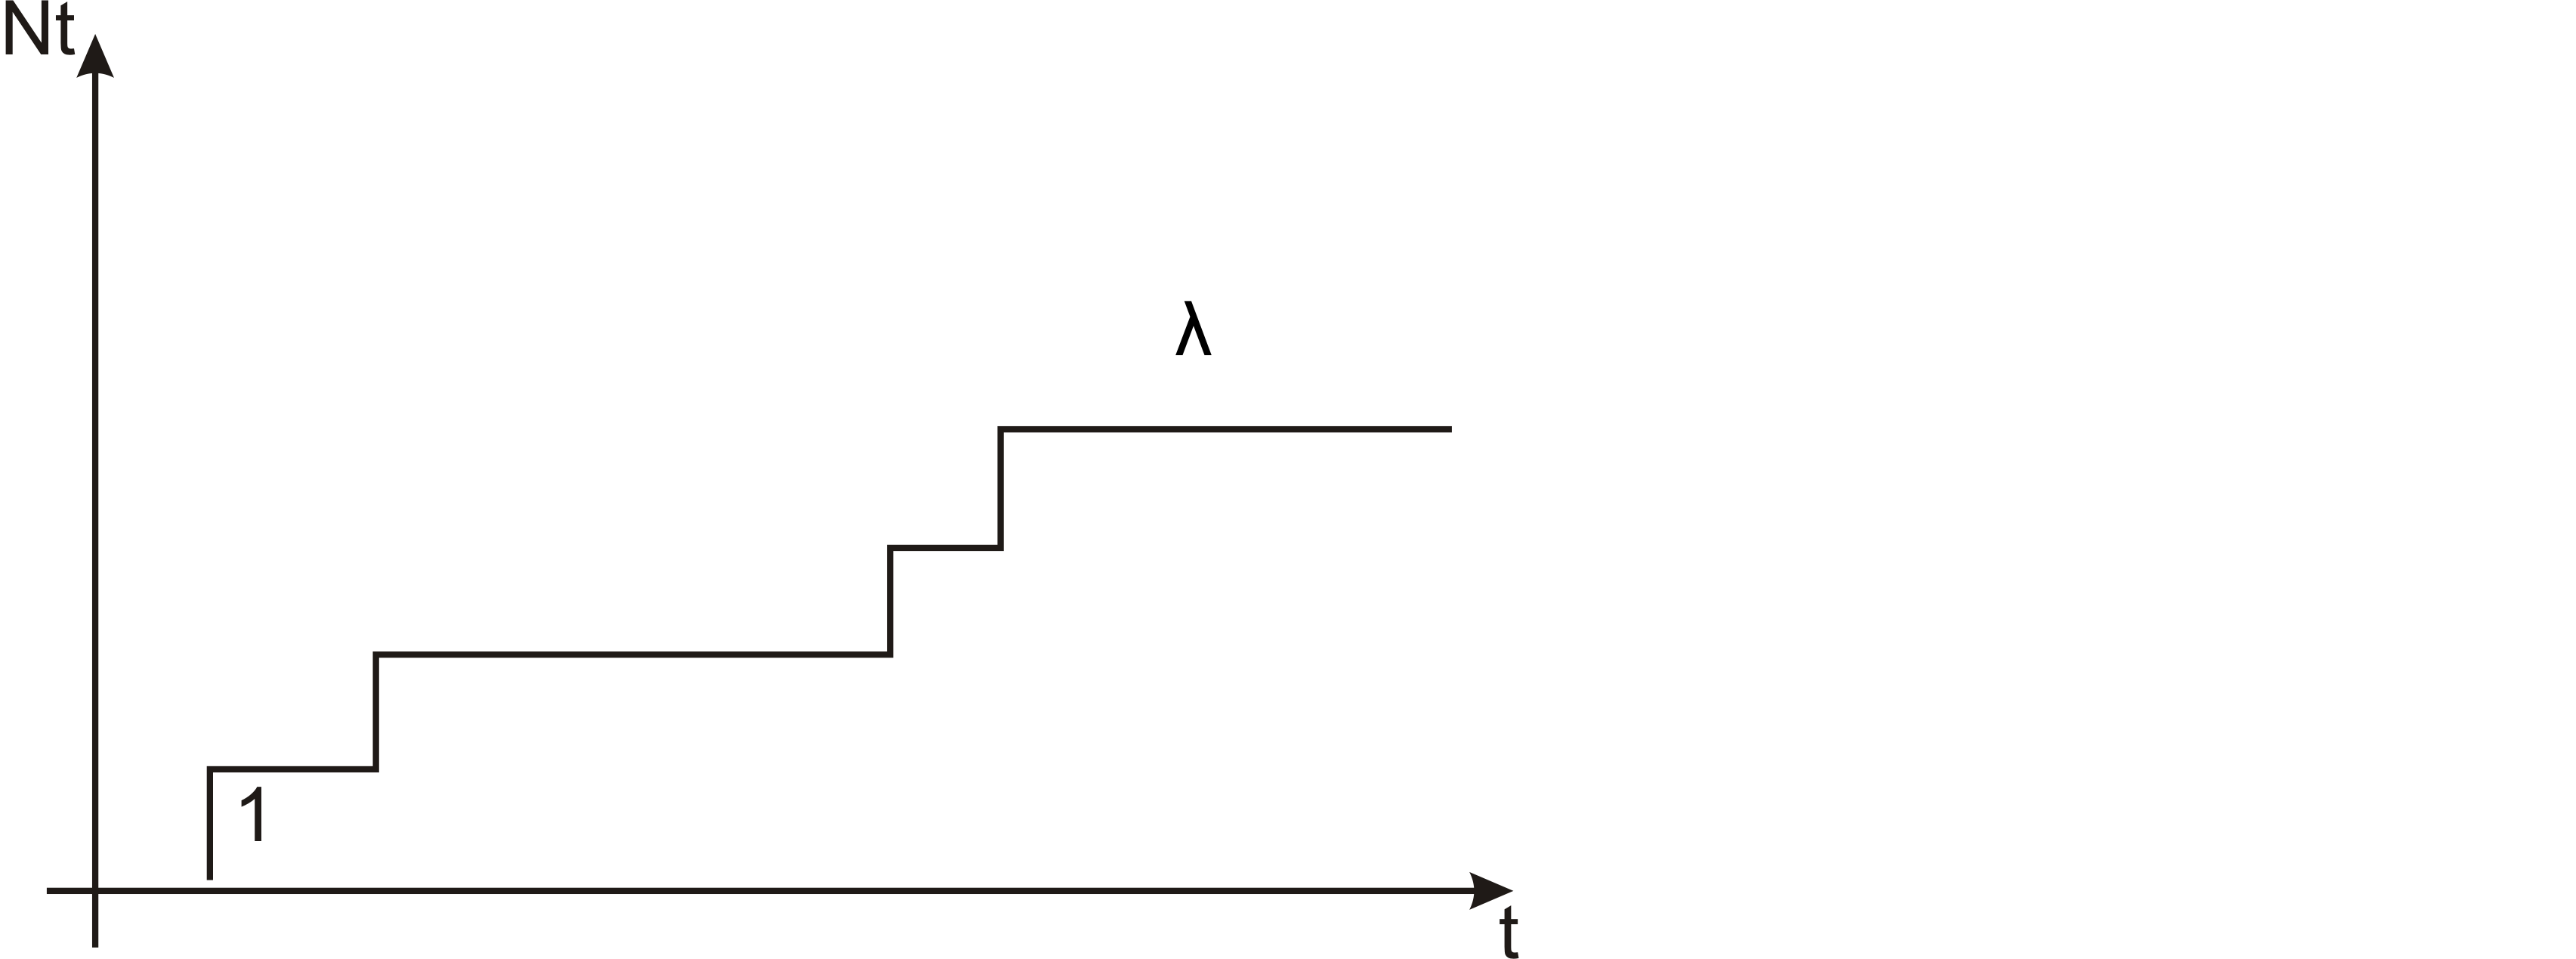
\includegraphics[width=4.5in]{Figures/rate.PNG}\\
%% \caption{}\label{}
%\end{figure}
%Suppose $\{N_{t}, t \geq 0\}$ Poisson process with rate $\lambda$. 
%
%$\tilde{N_{t}}(w)= N_{t}(w)+f(t+X_{1}(w))$ where $f(t)$=0, if $t$ is irrational and $f(t)$=t, if $t$ is rational.\\
%\begin{eqnarray*}
%% \nonumber to remove numbering (before each equation)
%P[\tilde{N_{t}}\neq N_{t}] &= P[\omega:t+X_{1}(\omega) \text{is rational}],\\
%&= P[\omega:X_1(\omega)  \text{is rational} ] =0.
%\end{eqnarray*}


\section{Non-Homogeneous Poisson Process}
From the characterization of Poisson process just stated, we can generalize to non-homogeneous Poisson process. In this case, the rate of Poisson process $\lambda$ is time varying. It is not clear from the first two characterizations, how to generalize the definition of Poisson process to the non-homogeneous case. We used third characterization of Poisson process for this generalization. 

\begin{defn}[Non-Homogeneous Poisson Process]\label{defn:NonHomogeneousPoisson} A point process $\{N(t),~t\geqslant 0\}$ is said to be \textbf{non-homogeneous Poisson process} with instantaneous rate $m(t)$ if it has stationary independent increments, and 
	\begin{eqnarray*}\label{eq:NonHomogeneousPoisson}
		\Pr\{N(t)=0\}&=&1-m(t)+o(t). \\
		\Pr\{N(t+\delta)-N(t)=0\} &=& 1-m(t)\delta+o(\delta). \\
		\Pr\{N(t+\delta)-N(t)=1\} &=& m(t)\delta+o(\delta). \\
		\Pr\{N(t+\delta)-N(t)>1\} &=& o(\delta). \\
	\end{eqnarray*}
\end{defn}

\begin{prop}[Non-Homogeneous Distribution] Distribution of non-homogeneous Poisson process $N(t)$ with instantaneous rate $m(t)$ is given by
	\begin{align*}
		\Pr\{N(t)=n\}=\frac{(\bar{m}(t))^n}{n!}e^{-\bar{m}(t)},
	\end{align*}
	where $\bar{m}(t)$ is the cumulative rate till time $t$, i.e. $\bar{m}(t)=\int_{0}^{t}m(s)ds$. 
\end{prop}
\begin{proof}
	Let's denote $f(t) = \Pr\{N(t)=0\}$. Further, from independent increment property of $N(t)$, we notice that $\{N(t+\delta) = 0\}$ is intersection of two independent events given below, 
	\begin{align*}
		\{N(t+\delta)=0\} \iff \{N(t)=0\}\cap\{N(t+\delta)-N(t)=0\}.
	\end{align*}
	From Definition~\ref{defn:NonHomogeneousPoisson}, it follows that
	\begin{align*}
		f(t+\delta) = f(t)[1 - m(t)\delta + o(\delta)].
	\end{align*}
	Re-arranging the terms in the above align, dividing by $\delta$, and taking limit as $\delta \downarrow 0$, we get 
	\begin{align*}
		f'(t) = -m(t)f(t).
	\end{align*}
	Since $f(0) = 1$, it can be verified that $f(t) = \exp(-\bar{m}(t))$ is solution for $f(t)$.
	%\begin{eqnarray*}
	%f(t+\triangle) &=& \Pr\{N_{t+\triangle}=0] \\
	%&=&  \Pr\{N(t)=0, N_{t+\triangle}-N(t)=0]\\
	%&\stackrel{(a)}{=}& \Pr\{N(t)=0] \Pr\{N_{t+\triangle}-N(t)=0]\\
	%&=& f(t)[1-m(t)\triangle +o(\triangle)].\\
	%\frac{f(t+\triangle)-f(t)}{\triangle} &=& -m(t) f(t) +f(t) \frac{0(\triangle)}{\triangle}. \\
	%\lim_{\triangle\downarrow 0}\frac{f(t+\triangle)-f(t)}{\triangle} &=& -m(t) f(t) \\
	%\frac{d f(t)}{t} &=& -m(t) f(t),  \\
	%\end{eqnarray*}
	%where (a) follows from independent increment property. Since, $\overline{m}(t)=\int ^{t}_{0} m(s) ds $, $f(t)=\Pr\{N(t)=0]$, $ f(0)=\Pr\{N_{0}=0] =1$ the solution of the differential align can be verified to be $f(t)=e^{-\overline{m}(t)}$, as follows: 
	%\begin{eqnarray*}
	%f(0)&=& e^{-\overline{m}(t)}\\
	%&=& e^{-0}=1 \\
	%f'(t) &=& e^{-\overline{m}(t)}\frac{d}{dt} \int^{t}_{0}m(S) ds\\
	%&=& m(t)e^{-\overline{m}(t)}, t\geqslant 0 \\
	%\end{eqnarray*}
	%
	%\begin{eqnarray*}
	%\Pr\{N_{t+\triangle}-N(t)=0] &=& 1-m(t)\triangle +o(\triangle) \\
	%\Pr\{N_{\triangle}-N_{0}=0] &=& 1-m(0)\triangle +o(\triangle) 
	%\end{eqnarray*}
	%Since $ N_{0}=0$, 
	%\begin{eqnarray*}
	%\Pr\{N_{\triangle} =0]&=& 1-m(0)\triangle +0(\triangle) \\
	%\lim_{\triangle\downarrow 0}f(\triangle) &=& f(0)=1.
	%\end{eqnarray*}
	We have shown $\Pr\{N(t)=0\} = \exp(-\bar{m}(t))$. By induction, we can show the result for any $n$.
\end{proof}

\end{document}